\documentclass[11pt,letterpaper]{article}
\usepackage{inputenc}
\usepackage{amsmath}
\usepackage{amsfonts}
\usepackage{amssymb}
\usepackage{graphicx}
\usepackage{enumitem}
\usepackage{fancyhdr}
\usepackage{tikz}
\usepackage{hyperref}
\usepackage[T1]{fontenc}
\usepackage{graphicx}
\usepackage{color}
\usepackage{bm}
\usepackage{ mathrsfs }
\usepackage{multirow}
\usepackage{subcaption}
\usepackage{relsize}
\usepackage{algorithm}
\usepackage[noend]{algpseudocode}
\usepackage[backend=bibtex]{biblatex}
\definecolor{lightgray}{gray}{0.5}
\setlength{\parindent}{0pt}
 \usepackage[top=3cm, bottom=2cm, left=1.9cm, right=1.9cm]{geometry}

% \usepackage[table,xcdraw]{xcolor}
\usepackage{xcolor}
\colorlet{qblue}{blue!50!black}
\colorlet{lblue}{blue!50!black}
\colorlet{fblue}{blue!60!black}
\colorlet{fred}{red!60!black}
\DeclareGraphicsExtensions{.pdf,.png}


\usepackage{algorithm}
\usepackage[noend]{algpseudocode}
\usepackage{booktabs}
%{\renewcommand{\arraystretch}{1.2}
\newcommand{\comment}{\algorithmiccomment}
\DeclareMathAlphabet{\mathcal}{OMS}{cmsy}{m}{n}
%\newcommand{\captionsize}{\normalfont}
%\newcommand{\captionfont}{\captionsize}
%\usepackage{verbatimbox} %BB-AY this breaks my TeX setup
\usepackage{placeins}
% for fortran code listings
\bibliography{eecs587.bib}

\pagestyle{fancy}
\renewcommand{\headrulewidth}{1pt}
\title{Accelerating the Computation of Geometric Constraints in Optimization}
\author{Benjamin J. Brelje}
\lhead{Benjamin J.~Brelje}
\chead{EECS587 Term Project}
\rhead{\today}
\begin{document}

\maketitle

\section{Introduction}
\qquad In aerospace engineering, particularly in commercial aviation, reducing cost and environmental impact is a major research focus.
My lab, the Multidisciplinary Design Optimization Lab (MDOLab), uses numerical optimization and computer simulation to create aircraft designs with minimum fuel consumption.
The output of one of our optimizations is an aircraft geometry file.

\qquad Previous graduate research resulted in efficient, massively parallel flow solvers and structural analysis tools.
These tools allow us to assess the weight and drag of a particular geometry.
The optimizer will run many of these aerostructural analyses until it converges on the optimal design.

\qquad Another important aspect of aircraft design is geometric constraints.
An example of a geometric constraint is that the aircraft must have enough volume in the wing for the mission's required fuel.
The focus of my research is making realistic geometric constraints easier to impose on our optimization problems.
In my previous work, I developed a Python package called \texttt{geograd} to compute the value of my new geometric constraints during optimization.
\texttt{Geograd} uses Tensorflow, a framework designed for machine learning, to compute my constraint in a pure SIMD fashion.
It was very fast when running on the GPU on my local machine, but we do not have access to GPU resources on our usual compute clusters.
The purpose of this term project is to greatly improve the performance of \texttt{geograd} by writing a brand-new, Fortran 90 implementation to take advantage of algorithm opportunities that cannot be posed in Tensorflow's SIMD language.

\qquad The first section will describe the specific computation in more detail and the current state of the software.
Second, I will describe a test case I constructed for my timings and benchmarking.
Following that, I will describe the development and verification of my baseline Fortran code.
Next, I will walk through each improvement I made to the algorithm and describe the dynamic load balancing problem that emerged during this step.
Finally, I will describe the dynamic load balancing approach I used and present the final timings.

\qquad I was ultimately able to achieve over a 1350x speedup on my benchmark case compared to my original Tensorflow-based pure SIMD implementation.

\section{Description of the Computation and Previous Work}
In numerical optimization, algorithms are designed to minimize some objective function $f(\textbf{x})$ by varying $\textbf{x}$ (a vector of design variables)
subject to $\textbf{g}(\textbf{x}) \leq 0$ (a vector of constraint values).
In aircraft optimization:
\begin{itemize}
 \item $f(\textbf{x})$ is generally fuel burn for a given mission
 \item $\textbf{x}$ are geometric parameters like wingspan, wing sweepback angle, and local thickness control points
 \item $\textbf{g}(\textbf{x})$ includes structural stress limits, stall speed requirements, and other requirements.
\end{itemize}
My research goal is to define a mathematical formulation for a component of $\textbf{g}$ which accounts for geometric constraints due to packing.
Notionally, my constraint $\textbf{g} \leq 0$ when the item I need to package fits entirely within the outer envelope of the airplane.

\qquad Our lab uses \emph{gradient-based} optimization because we have many (hundreds) of design variables $\textbf{x}$.
Optimization algorithms which use gradient information are computationally cheaper than gradient-free methods on large-scale problems like ours.
When I say \emph{gradient information}, I am referring to the derivatives of the objective and constraints with respect to the design variables, namely:

\begin{equation}
    \frac{df(\textbf{x})}{d\textbf{x}}
\end{equation}

\begin{equation}
    \frac{d\textbf{g}(\textbf{x})}{d\textbf{x}}
\end{equation}

\qquad While gradient-based methods require orders of magnitude fewer function evaluations on large-scale problems, they require the researcher to define computational methods which include both function values and derivatives.
They also introduce requirements on the general behavior and smoothness of the functions.
Obviously, $f$ and $\textbf{g}$ must be once-differentiable.
Gradient-based methods perform best when $f$ and $\textbf{g}$ are deterministic.
Ideally, $f$ and $\textbf{g}$ are also $C^1$ continuous (smooth values and first derivatives), though adequate results can also be obtained with $C^0$ continuous functions (smooth values only) in some cases.

\qquad During the course of my research, I identified a mathematical formulation for a geometric constraint which meets these requirements.
We begin with triangulated representations of aircraft outer surface $r$ and an inner object $s$ to pack inside it, as pictured in Figure~\ref{fig:schematic}.
$r$ and $s$ are each represented as lists of vertices $\textbf{A}$, $\textbf{B}$, $\textbf{C}$ of dimension 3 by $m$ or $n$ (the size of each mesh).

\begin{figure}[ht]
  \centering
  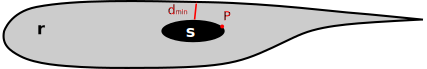
\includegraphics[width=0.45\linewidth]{figures/schematic}
  % \vspace{-30pt}
  \caption{A section view of an object $s$ inside wing $r$ and the minimum distance $d_\text{min}$ between them}
  \label{fig:schematic}
\end{figure}

\qquad When one object encloses another, the minimum distance $d_\text{min}$ between them is greater than zero by some margin.
Therefore, a first approach to a geometric constraint might involve computing $d_\text{min,rs} \geq 0 + \text{tol}$.
We can compute $d_\text{min}$ between two triangulated surfaces by computing the minimum distance between each individual pair of triangles.
The minimum distance between a pair of triangles can be found by a total of fifteen primitive tests between the vertices: six point-triangle tests, and nine line-line tests (Figure~\ref{fig:primitives}). % TODO cite ericson

\begin{equation}
  \label{eq:dmin}
  d_\text{min,rs} = \text{min}(d_{\text{min},ij}) \text{ for each triangle } i, \, j \text{ in surfaces } r, \, s
\end{equation}

\begin{figure}[ht]
  \begin{subfigure}[b]{0.48\textwidth}
    \includegraphics[width=\textwidth]{figures/point-tri.pdf}
    \caption{Six point-tri tests}
    \label{fig:point-tri}
  \end{subfigure}
  \hfill
  \begin{subfigure}[b]{0.48\textwidth}
    \includegraphics[width=\textwidth]{figures/edge_edge.pdf}
    \caption{Three of nine line-line tests}
    \label{fig:line-line}
  \end{subfigure}
  \caption{Geometric primitive tests between facet $i$ of the outer surface and $j$ of the component}
  \label{fig:primitives}
\end{figure}

\qquad During optimization, the pair of facets comprising the minimum distance can change rapidly, leading to discontinuities in the gradients and poor optimizer performance.
Notionally, we want to gather information not only from the exactly closest triangles, but also from the triangles that are nearly closest.
We can achieve this by using a strategy called constraint aggregation.
I used a function called the Kreisselmeier-Steinhauser (KS) function which essentially provides a conservative estimate of the extremum of a vector.
The computation is as follows:

\begin{equation}
  \label{ks_geom}
  KS_\text{geom}(\textbf{x}) = \frac{1}{\rho} \textrm{ln} \Bigg[\sum_{i,j=1}^{m,n} e^{\rho\big(d_\text{min}\:(\textbf{x})-d_{ij}\:(\textbf{x})\big)}\Bigg] - d_\text{min}\:(\textbf{x}) \leq 0 ,
\end{equation}

where $\textbf{x}$ is a vector of design variables,
$d_{ij}(\textbf{x})$ is the pairwise distance between the $i$th facet of $r$ and $j$th facet of $s$,
$d_{min}(\textbf{x})$ is the minimum distance between $r$ and $s$ at the current design point, and
$\rho$ is a user-controllable constant.
Strictly speaking, $d_{ij}$ is a function of the surface mesh points of $r$ and $s$, not the design variables $\textbf{x}$ directly.

\qquad Last year, I implemented the computation of Equation~\ref{ks_geom} using the Tensorflow framework. % cite tensorflow
Tensorflow is a Python package designed for machine learning, originally developed by Google.
Tensorflow uses a graph representation of a series of array operations and computes a result in a SIMD fashion.
Since many machine learning workflows require gradients for training purposes, Tensorflow natively supports analytic reverse-mode derivatives, making it ideal for use in gradient-based optimization.
Tensorflow also supports heterogeneous computer architectures, including GPU acceleration.
I found that I could run the calculation almost instantaneously on the GPU of my desktop machine.

\qquad I used my implementation, which I call \emph{geograd} (for ``\emph{geo}metric constraints with \emph{grad}ients''), for several published optimization studies over the last 12 months. %cite scitech, aviation papers
To run the published optimization cases, I used the Texas Advanced Computing Center (TACC) Stampede2 cluster.
Unfortunately, while TACC does have GPU nodes, the geometry calculation is a very small portion of the overall compute cost (which includes expensive, CPU-based fluid dynamics calculations).
Therefore, it did not make economic sense to reserve GPU nodes just for the geometry constraints since it would be idle a large percentage of the time.

\qquad Instead, I used Tensorflow's CPU support and created an optimized, CPU-parallel implementation.
I used the \texttt{mpi4py} package to scatter the computation over all MPI processes, run one Tensorflow call on each process, and gather the results.
I built Tensorflow from source with Intel MKL support and architecture-specific optimizations, including the Intel AVX-512 SIMD extensions.
This confguration provided enough performance for my immediate research needs, but increased the wall time significantly compared to the GPU card on my desktop.
I need to reduce the computation time in order to scale up to more complex optimization problems with more objects to pack inside the airframe.

\qquad Tensorflow's SIMD approach makes it infeasible to use control flow and early exits to reduce the cost of the geometry calculations, which results in a large number of redundant calculations.
I brainstormed several potential approaches which can be used to reduce compute cost, including:
\begin{itemize}
  \item Arranging control flow so that the most likely branches are tested first
  \item Using the minimum instead of the sum of the 15 pairwise primitives for each triangle (reduces the gradient compute cost by 15x)
  \item Using bounding box tests to quickly exclude pairs of facets which are far away from each other and cannot possibly be the minimum distance
\end{itemize}
In order to use these approaches, I need control flow.
Therefore, I need to drop the Tensorflow SIMD formalism and write my own CPU-optimized implementation in Fortran with Python bindings.
The term project consists of this new Fortran 90 implementation.

\section{Benchmarking Case Description}
\label{sec:benchmark}
\qquad I wanted to isolate performance metrics to the geometry code, yet test the code in a setting representative of an optimization run, so I generated an artificial test problem.
Consider a blended wing body (BWB) aircraft, as pictured in Figure~\ref{fig:bwb-alone}.
We might optimize the shape of this aircraft to minimize drag.
Aircraft also need to hold systems components (such as actuators and hydraulic pumps).
I created a notional football-shaped geometry to represent a generic system component to be packed optimally into the wing and placed it into the right wing root, as pictured in Figure~\ref{fig:bwb-blob}.
We can then compute Equation~\ref{ks_geom} between the aircraft outer shape $r$ and the football-shaped inner component $s$ to see whether the current layout is feasible.

\begin{figure}[ht]
  \centering
  \includegraphics[width=0.66\linewidth]{figures/bwb_alone.png}
  \caption{This blended wing body geometry was used for the test problem}
  \label{fig:bwb-alone}
\end{figure}

\qquad During optimization, the relative positions of the two objects will change.
Generally, the changes in position will be fairly subtle.
However, to make the test problem as challenging as realistically possible, the component translates from one wing root to the other in 50 equally-spaced increments.
The arrow in Figure~\ref{fig:bwb-blob} shows the path of the component.
The test comprises computing Equation~\ref{ks_geom} 50 times, one at each component position.
I implemented the test as a Python unittest file (\texttt{test\_speed.py} in the repository).
Two timings are obtained; one for analysis only (no gradient), and another with gradients.

\begin{figure}[ht]
  \centering
  \includegraphics[width=0.80\linewidth]{figures/bwb_With_blob_arrow.png}
  \caption{The component geometry translates from one side of the aircraft to the other in the test problem}
  \label{fig:bwb-blob}
\end{figure}

\section{Baseline Code Development and Verification}
\qquad Because this code will be used to produce published research results, I need to ensure the code is not only fast, but also accurate.
I developed the code in the following general steps:
\begin{itemize}
  \item Writing line-line and point-triangle test primitive subroutines
  \item Algorithmic differentiation of the geometric primitives
  \item Writing the serial KS function subroutine (implementing Equation~\ref{ks_geom})
  \item Creating the Python-Fortran interface
  \item Unit testing of the geometric primitives and KS function
  \item Parallelizing the KS function subroutine
\end{itemize}

\subsection{Writing Geometric Primitives}
\qquad I implemented the line-line and point-triangle tests as described in Ericson. % TODO cite ericson
The subroutines, contianed in \texttt{triangles.F90} take four three-dimensional points as input and return the minimum distance.
The sequence of control flow is designed to exit early in some common cases, deferring the least likely paths until as late as possible.
I also developed unit tests using triangles in prescribed configurations to exercise each of the branches of the mathematics.

\subsection{Algorithmic Differentiation of the Primitives}
\qquad We not only need to know the minimum distance result of the primitives; we also need the derivatives with respect to the function inputs.
It is possible to derive this by hand; however, it is much easier to use source code transformation via algorithmic differentiation (AD).
I differentiated the point-triangle and line-line primitive subroutines using the \href{https://www-sop.inria.fr/tropics/tapenade.html}{INRIA Tapenade} software.
There are two modes in AD: forward and reverse (also known as backprop).
I used reverse mode, which requires only one function evaluation to get the derivatives of a single output ($d_{min}$) with respect to all 12 of the inputs (four points, three dimensions each).

\subsection{Assembling the KS Function and Gradients}
\qquad I implemented the loops to compute Equation~\ref{ks_geom} with respect to all of the $m$ facets of an outer surface and $n$ facets of the inner surface.
The subroutine \texttt{compute} takes 8 inputs:

\begin{itemize}
  \item $A_r$, $B_r$, $C_r$: lists of vertices comprising the $m$ triangles of the outer surface
  \item $A_s$, $B_s$, $C_s$: lists of vertices comprising the $n$ triangles of the inner object surface
  \item $d_\text{min,current}$: the minimum distance between the two surfaces at the current design point (this is used to normalize the calculation which improves numerical conditioning)
  \item $\rho$: a user-defined constant which defines how tight the objects can fit next to each other
\end{itemize}

The subroutine returns:

\begin{itemize}
  \item $KS$: the constraint described in Equation~\ref{ks_geom}
  \item $d_\text{min}$: minimum distance between the two surfaces
\end{itemize}

The major advantage that this Fortran implementation has over Tensorflow is data reuse.
Tensorflow computes each array operation in a pairwise fashion sequentially.
Every entry in each array is read one time per array operation, and one write is performed per array operation.
This should result in a bad compute-to-memory access ratio.
In the Fortran implementation, each pair of triangles is read from the global arrays only one time.
Subsequently, all the primitive tests and summation is performed on local copies which should easily fit in the L1 cache.
This should result in a major speedup over the Tensorflow implementation by itself.

I was careful to ensure sequential memory access by arranging the array order correctly.
Fortran uses column-major order, so I used the spatial dimensions $x,y,z$ as the first array dimension, and triangle count $i,j$ as the second dimension.
This results in coalesced memory access when individual vertices are read from the global arrays.
However, for the purposes of visualization in this paper, I illustrate the transpose of the matrix, with each row comprising a triangle.

I also wrote a function \texttt{compute\_derivs} which additionally computes the following derivatives with respect to the surface mesh points (all $m$ by 3 arrays):

\begin{equation}
  \frac{dKS}{d\textbf{A}_r} \, \, \, \, \, \, \frac{dKS}{d\textbf{B}_r} \, \, \, \, \, \, \frac{dKS}{d\textbf{C}_r}
\end{equation}

and the following derivatives with respect to the object mesh points (all $n$ by 3 arrays):

\begin{equation}
  \frac{dKS}{d\textbf{A}_s} \, \, \, \, \, \, \frac{dKS}{d\textbf{B}_s} \, \, \, \, \, \, \frac{dKS}{d\textbf{C}_s}
\end{equation}

These derivatives are required in order to compute the total derivative of the KS function with respect to the design variables.
Recall that Equation~\ref{ks_geom} depends on the surface mesh vertices $A$, $B$, and $C$ of objects $r$ and $s$.
Applying the chain rule, we have:

\begin{equation}
  \frac{dKS}{d\textbf{x}} = \frac{dKS}{d\textbf{A}_r(\textbf{x})} \frac{d\textbf{A}_r(\textbf{x})}{d\textbf{x}} +
                            \frac{dKS}{d\textbf{B}_r} \frac{d\textbf{B}_r}{d\textbf{x}} +
                            \frac{dKS}{d\textbf{C}_r} \frac{d\textbf{C}_r}{d\textbf{x}} +
                            \frac{dKS}{d\textbf{A}_s} \frac{d\textbf{A}_s}{d\textbf{x}} +
                            \frac{dKS}{d\textbf{B}_s} \frac{d\textbf{B}_s}{d\textbf{x}} +
                            \frac{dKS}{d\textbf{C}_s} \frac{d\textbf{C}_s}{d\textbf{x}}
\end{equation}
We have a separate Python tool which provides the design variable sensititivies $d\textbf{A,B,C}/d\textbf{x}$.


\qquad Differentiating top-level code, particularly when it involves dynamically-allocated arrays or MPI calls, can be very inefficient.
Therefore, I differentiated Equation~\ref{ks_geom} by hand, obtaining:

\begin{equation}
  \frac{dKS}{d\textbf{A}_r} = -\frac{\mathlarger{\sum_{i,j=1}^{m,n} \frac{d\,d_{ij}}{d\textbf{A}_r}e^{\rho\big(d_\text{min}-d_{ij}\big)}}}
  {\mathlarger{\sum_{i,j=1}^{m,n} e^{\rho\big(d_\text{min}-d_{ij}\big)}}}
\end{equation}

and so on for the remaining 5 lists of input vertices.
$d\,d_{ij}/d\textbf{A}_r$ is computed using the AD version of the geometric primitives.

\qquad Note that, while $dKS/d\textbf{A}_r$ is a dense $m$ by 3 matrix, each pairwise update in the summation ($d\,d_{ij}/d\textbf{A}_r$) is sparse and affects at most 3 entries at a time.
Note also that the summation in the denominator is a global quantity, while the numerator is a local quantity specific to each facet pair $i$,$j$.
Since the entries of the derivatives depend on both local information as well as the global summation across all the facet pairs, the overall computation is not embarassingly parallel.
However, the amount of communication required is fairly low (a single partial sum is Allgathered from all processes) in between two separate double $ij$ loops.

\subsection{Fortran-Python interface}
\qquad The lab's optimization framework is Python-based.
Therefore, all geometry information fed into the Fortran code needs to be passed in from a Python process executed under MPI.
Normally, writing Python native interfaces is a royal pain, and in the past I have used the low-level Python-C API to do this.

\qquad A better way is to use the \texttt{f2py} interface generator.
\texttt{f2py} was developed as part of the \texttt{numpy} project and it is distributed with \texttt{numpy}.
It consists of a command-line interface which reads and compiles Fortran source and generates a \texttt{.so} shared object file which can be imported as a Python package.
The user can control the structure of the input and output arguments by writing an f2py ``signature'' file, which I did in this case.
F2py passes in numpy arrays by reference as native Fortran array pointers in the correct column-major memory layout.

\qquad The build process can be pretty involved, so I created a Makefile for the project.
The default ``make'' command line argument on Linux should successfully compile and test the entire project, assuming the proper dependencies are already installed.

\subsection{Testing and Verification}
\qquad A major benefit of the Python interface is that it is easy to create unit and integration tests.
As I developed the codebase in a bottom-up approach, I ensured that unit tests were written and passing before moving on.
First, I generated unit tests which cover every branch of the geometry primitives using simple configurations of triangles (\texttt{test\_primitives.py}).
Next, it is absolutely crucial to test the accuracy of AD derivatives, since Tapenade sometimes can be buggy and these types of errors can be difficult to detect in integration testing.

\qquad In order to verify derivatives, we use the \emph{complex step} method (CS).
The complex step method (Equation~\ref{eq:complex_step}) is conceptually similar to finite differencing, except that it is exactly accurate even when a very small step (on the order of machine $\epsilon$) is used.
This makes it suitable for testing the exact derivatives obtained via AD to high precision.

\begin{equation}
  \label{eq:complex_step}
  \frac{df(x)}{dx} = \frac{\text{Im}(f(x+ih))}{h}
\end{equation}

\qquad The drawback of the complex step method is that it requires that the code being tested support complex inputs.
Fortunately, our lab has developed a method for compiling complex versions of our Fortran codes.
We use a Python script to transform the base code into a complexified version.
The script changes data types and overloads certain functions so that they produce the correct control flow even with complex inputs.
I added this complex build to the Makefile and wrote unit tests verifying the derivatives of both the geometric primitives as well as the top-level KS function derivatives.
All the derivative outputs matched CS to a relative tolerance of $10^{-7}$, indicating that both the AD derivatives and the by-hand derivative assembly were correctly implemented.

\qquad Finally, I ported my previous integration tests from \texttt{geograd} over to this project and verified that the output values match the output values of my new code for known geometries.
They did match to a high degree of accuracy.

\subsection{Parallelizing the Baseline Code}
\qquad As a first cut, I parallelized the new Fortran code in the same way that I had parallelized \texttt{geograd}.
Here are the assumptions and requirements for the parallelization:
\begin{itemize}
  \item Assume each process has a full copy of the input meshes $r$ and $s$ when it is called (no scatter from root required)
  \item Each process must end up with a full copy of both the KS value and all the derivative arrays
  \item The $p$ processors will be provisioned such that $p >> m, n$
\end{itemize}
We divide up the problem along the $r$ mesh only.
Each processor is given a range of rows in the $r$ mesh arrays to compute against all of the $s$ triangles.
Figure~\ref{fig:parallel} shows the parallelized arrangement.
First, an owner-computes approach is used to compute the summation of the KS function.
Each process recieves the summation value via an allreduce.
If analysis is being performed without the need for derivatives, the computation is done at this point.
If not, the derivatives are computed in an owner-computes fashion.
Since the processors ``share jurisdiction'' over the $s$ mesh, an MPI Allreduce summation is used to combine local copies of the $s$ derivatives into a global array.
The $r$ mesh is simply concatenated and sent to all using the MPI Allgather subroutine.

\begin{figure}[ht]
  \centering
  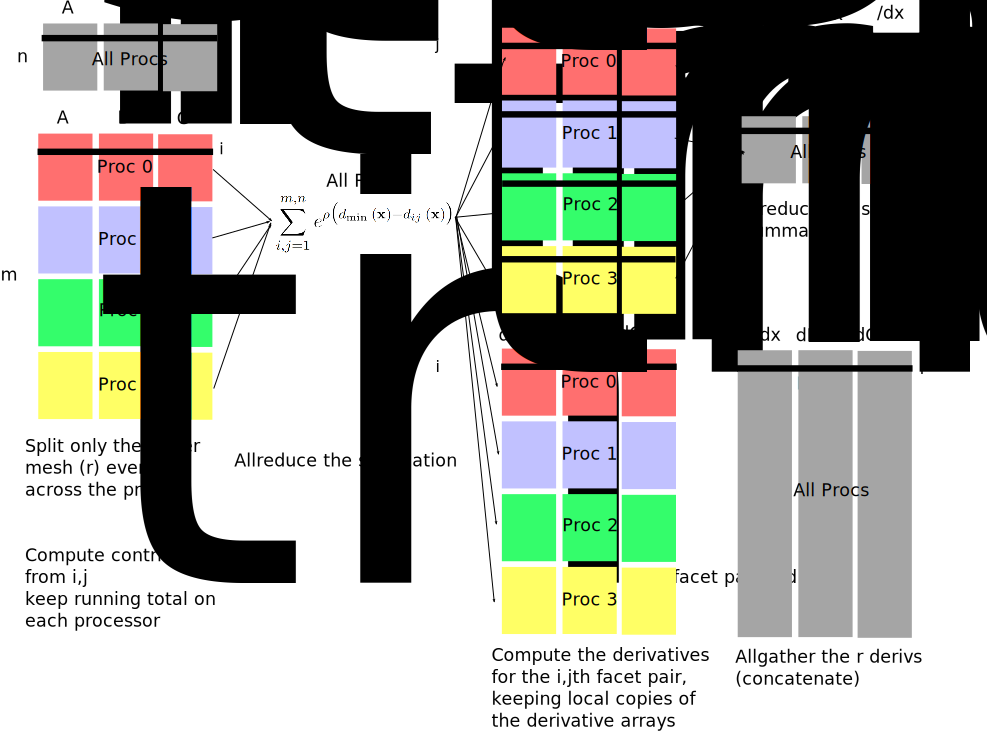
\includegraphics[width=0.95\linewidth]{figures/parallelization}
  \caption{The problem is parallelized by dividing up the larger array and distributing its computation evenly across the processors}
  \label{fig:parallel}
\end{figure}

\subsection{Timing the Baseline}
I ran the \texttt{geograd} (Tensorflow-based) implementation and my new Fortran implementation on the benchmark problem described in Section~\ref{sec:benchmark} using 4 to 48 cores of a compute node on the TACC Stampede2 cluster.
Unless otherwise specified in the report, I give timings and speedups for the 48-core case.
The Tensorflow-based benchmark took 20s to run analysis only, and 38s for derivatives.
My new Fortran-based benchmark took 0.371s for analysis only (\textbf{53x} speedup), and 1.93s for derivatives (\textbf{19x} speedup).
These were extremely promising results, and I had not yet implemented any of the algorithm improvements.

\section{Algorithm Improvements}
Because Tensorflow does not support control flow (at least, not in a form which reduces computation for unused branches), there is great opportunity to gain speed by improving the algorithm.
In this section I describe the improvements and report speedup relative to the previous iteration (not cumulative versus the original Tensorflow implementation).

\subsection{Minimum instead of Sum of the 15 Triangle Tests}
Recall the 6 point-triangle and 9 line-line tests performed for each pair $i,j$ of triangles, as shown in Figure~\ref{fig:primitives}.
In Tensorflow, there is no computational advantage to taking the minimum value of the 15 pairwise primitive tests, so I sum the KS results instead.
However, in Fortran, I can eliminate 14 of the 15 derivative calls by taking the minimum instead of the sum.
I added a case control flow structure to only run the derivative subroutine for the most critical primitive.
This had only a modest effect on the analysis-only benchmark (\textbf{1.1x} speedup), but a large effect on the derivatives benchmark (\textbf{3.93x} speedup).
This optimization remains an exactly correct expression of Equation~\ref{ks_geom}.

\subsection{Bounding Box Testing}
If a pair of triangles is far away from each other, it is possible to prove cheaply that their interaction is not important.
We can accomplish this through \emph{bounding box} testing.
Let's draw an axis-aligned bounding box around the inner object $s$ as pictured in Figure~\ref{fig:bb-test}.
Let us also define some tolerance value (say, the maximum dimension of $s$ in any dimension).
If the bounding box around triangle $j$ is more than $tol$ away from the bounding box of $s$, then we can guarantee that the minimum distance between them is at least $tol$.
We can then replace a potentially large number of $d_{ij}$ computations with $d_{ij}=tol$.

Computing bounding box tests is much cheaper than computing $d_{ij}$ using the subroutines.
The bounding box test is simply several min/max operations on each triangle $j$, plus a few floating point comparisons.
Since aircraft geometry predominantly varies in the wingspan direction, we can exclude a huge number of triangles with just one or two comparisons (by placing the $x$ axis tests first in the sequence).

I implemented the bounding box test using the heuristic $tol$ setting of $max(x_{max}-x_{min},\,y_{max}-y_{min},\,z_{max}-z_{min}$ and re-ran the benchmark cases.
The derivative benchmark gained an additional \textbf{3.4x} speedup compared to the previous optimization.

\begin{figure}[ht]
  \centering
  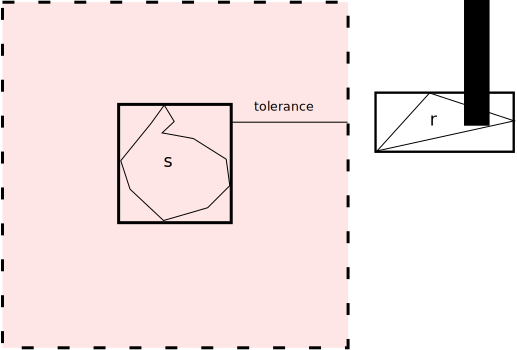
\includegraphics[width=0.65\linewidth]{figures/bb_test}
  \caption{Bounding box tests can quickly exclude obviously unimportant facets from needing expensive computation}
  \label{fig:bb-test}
\end{figure}

\section{Dynamic Load Balancing}
While the baseline Fortran implementation and the ``min of fifteen'' optimization had good load balancing (utilization above 95\% with 4 processors; above 65\% with 48 processors), the bounding box test absolutely ruined the load balancing.
The reason for this is spatial correlation in the lists of mesh vertices.
Consider the aircraft geometry pictured above.
A mesh representation might include all of the ``left wing'' triangles in the first quarter of the list, or it may be completely random (there are no guarantees).
A bounding box test excludes triangles that are far from the present position of the object $s$.
Therefore, if $s$ is in the right wing, the processor which is assigned all of the left wing facets may have zero triangles to compute.
Furthermore, as $s$ and $r$ deform and move during optimization, the load imbalance will change from processor to processor.

I measured this using the benchmarking case.
After implementing the bounding box test, my processor utilization across 48 MPI processes decreased from the high 60\% range to less than 15\%.
Examining the problem further, I found that one or two processors would have basically zero runtime, while the others were fully loaded.
I verified that these low-runtime processes had most or all of their triangles excluded from expensive tests by the bounding box.
Below, I will describe two approaches I used to solve the problem.

\subsection{Global Load Balancing}
Due to the dynamic nature of the load balancing issue, the load balancing step needs to be done on every function call.
As a first cut, I decided to treat the bounding box tests as negligible in cost and simply smear all of the ``active'' triangles (the ones passing the bounding-box test and requiring more expensive tests) evenly across the processors sequentially.
Briefly, the method is as follows:
\begin{itemize}
\item First, divide up all the triangles evenly across the processors
\item Compute bounding box tests and place a boolean into a local vector indicating whether it is active or inactive
\item Allgather the bounding box test results into a global vector on each processor
\item Compute the sum of all active triangles in the global vector
\item Compute a scan on the global vector to find the global indices $i$ of the triangles in $r$ across which the problem will be split for load balancing
\item Divide the triangles up across the new split indices
\end{itemize}
The structure of the problem remains as pictured in Figure~\ref{fig:parallel}, except that each processor will now have an unequal number of triangles to compute.
I chose to ignore the potential issue of some processors having more inactive (cheap) triangles to compute than others.
This keeps the array split indices limited in size and the split chunks contiguous in memory, which simplifies the collective operations required to get the derivatives assembled at the end.

This global load balancing method was very effective.
Processor utilization improved from about 11\% to 65\% (similar to the levels seen before implementing the bounding box tests).
The remaining idleness is attributable to some point-triangle or line-line tests being more expensive to compute than others (early exits, etc.), or to OS interrupts.
If the number of triangles per processor is high enough, load balancing improves to about 95\% (as in weak-scaling benchmark results).
With the load balancing in place, derivatives gained another \textbf{2.6x} speedup versus the unbalanced bounding box benchmark.
However, I noted that weak scaling seemed to suffer somewhat for this iteration.

After conducting some detailed profiling, I noted that the load balancing step was increasing in time as the number of triangles increased.
The reason was the MPI Allgather operation I used to construct the global load balancing vector.
My reasoning for this was to save bounding box test results so they wouldn't need to be recomputed later in the main loop.
However, it was clear that this would potentially cause poor scaling for larger problems.

\subsection{Distributed Load Balancing}
In order to eliminate the Allgather operation from the load balancing step, two changes were required.
First, I had to develop a distributed scan methodology to determine where the load balancing break indices would be located, without gathering a global vector of bounding box test results.
I was able to do this using an Allreduce operation with only as many values as processors, eliminating the weak scaling issue.
The second change was to insert the bounding box tests back into the main KS computation loop.
This resulted in doing some redundant bounding box tests, but they are so cheap that it barely matters.

I ran the benchmark for this distributed load balancing variant and found that the processor utilization remained equally high, and that the poor weak scaling of the load balancing step had disappeared.
Distributing the load balancing accounts for only about a \textbf{1.1x} speedup compared to the global load balancing, but it eliminates a sub-optimal scaling property that could come back to bite me in the future when working with larger problems.






\end{document}
